\documentclass[12pt,a4paper]{report}

% Encodage et langue
\usepackage[utf8]{inputenc}
\usepackage[T1]{fontenc}
\usepackage[french]{babel}
\usepackage[absolute,overlay]{textpos}


% Mise en page
\usepackage{geometry}
\geometry{left=2.5cm,right=2.5cm,top=2.5cm,bottom=2.5cm}
\usepackage{setspace}
\onehalfspacing

% En-têtes/pieds de page
\usepackage{fancyhdr}
\pagestyle{fancy}
\fancyhf{}
\lhead{Serpent}
\rhead{UNC - 2025}
\cfoot{\thepage}


% Maths et figures
\usepackage{amsmath, amssymb}
\usepackage{graphicx}
\usepackage[hidelinks]{hyperref}


% Pour la bibliographie simple
\usepackage{url}

\renewcommand{\thesubsection}{\arabic{subsection}}


\begin{document}

% Page de garde
\begin{titlepage}

    % --- Logo en haut à droite ---
    \begin{textblock*}{5cm}(15cm,0.5cm)
        
\includegraphics[width=5cm]{assets/logo.png} 
    \end{textblock*}

    % --- Titre justifié et limité ---
    \noindent
    \begin{minipage}{13cm}
        \raggedright
        {\scshape\Huge \textbf{Algorithme de chiffrement par bloc : Serpent} \par}
    \end{minipage}

    \vspace{0.5cm}

    \rule{\linewidth}{0.4pt}
    
    \vspace{0.1cm}

    \centering
    {\Large Rapport\par}

    \vspace{1.5cm}
    {\large NGUYEN Alexandre - MILLOT Nathan\par}

    \vspace{4cm}
    % --- Image du sujet ---
    \begin{center}
        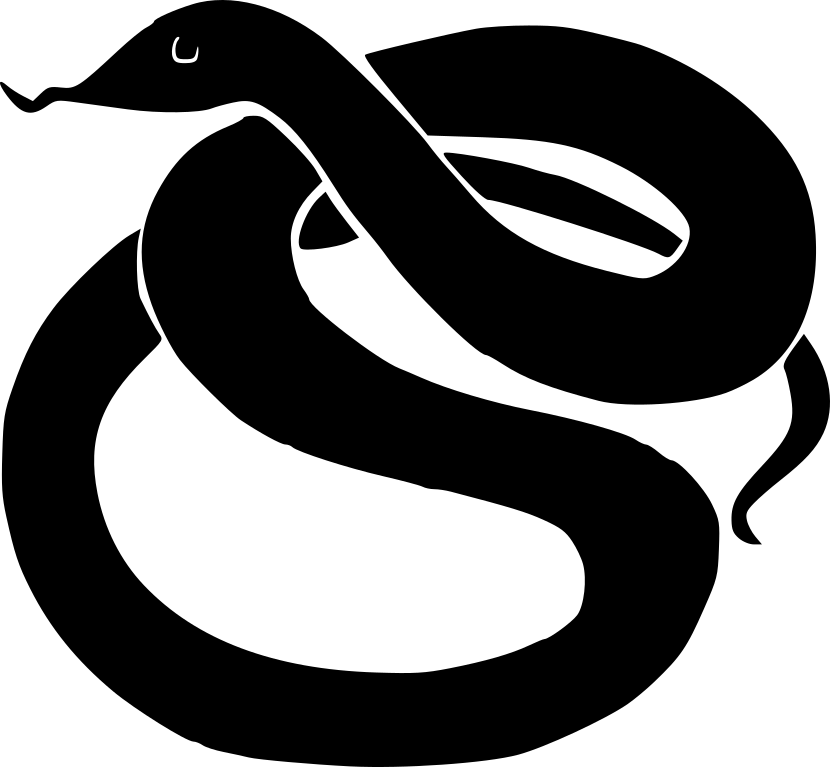
\includegraphics[width=0.5\linewidth]{assets/serpent.png}
    \end{center}

    \vspace{2.5cm}
    {\large Licence Informatique TREC 7  Semestre 6 \par}
   
    \vspace{1cm}
    {\large Date : \today \par}

\end{titlepage}

\tableofcontents










\section*{Introduction}
\addcontentsline{toc}{section}{Introduction}

Le chiffrement \textbf{Serpent} est un algorithme de chiffrement par bloc
conçu en 1998 par Ross Anderson, Eli Biham et Lars Knudsen dans le cadre du concours AES
(\textit{Advanced Encryption Standard}). Il a été finaliste, aux côtés de Rijndael, Twofish, MARS et RC6.

\section*{Espaces de définition}
\addcontentsline{toc}{section}{Espaces de définition}

\subsection{Messages en clair et chiffrés}
L’algorithme Serpent est un chiffrement par bloc avec :
\begin{itemize}
    \item Espace des messages en clair $M = \{0,1\}^{128}$ ;
    \item Espace des messages chiffrés $C = \{0,1\}^{128}$.
\end{itemize}
Chaque bloc est donc constitué de 128 bits.

\subsection{Clefs}
L’espace des clefs dépend de la taille choisie :
\begin{itemize}
    \item $K = \{0,1\}^{128}$ ;
    \item $K = \{0,1\}^{192}$ ;
    \item $K = \{0,1\}^{256}$.
\end{itemize}
En pratique, Serpent est défini pour ces trois tailles de clef.










\section*{Description du schéma Serpent}
\addcontentsline{toc}{section}{Description du schéma Serpent}

\setcounter{subsection}{0}

\subsection{Structure générale}
Serpent est basé sur un \textbf{réseau de substitution-permutation (SPN)}.  
Il comporte 32 tours successifs :
\begin{enumerate}
    \item Ajout de sous-clef (XOR avec la sous-clef de tour) ;
    \item Substitution via une des 8 S-boxes (non-linéarité) ;
    \item Transformation linéaire (permutation de bits).
\end{enumerate}
Avec un changement sur le $32^{\text{ème}}$ tour qui remplace la \texttt{Transformation linéaire} par un \texttt{Ajout de sous-clef} utilisant la $33^{\text{ème}}$ sous-clef ($K_{32}$).

\subsection{Sous-fonctions}

\subsubsection{Génération de sous-clefs}
À partir de la clef initiale, Serpent dérive 33 sous-clefs de 128 bits chacune, notées $K_0, K_1, \dots, K_{32}$.

\subsubsection{Substitution (S-boxes)}
Huit S-boxes différentes sont utilisées, notées $S_0, \dots, S_7$.  
Elles transforment des blocs de 4 bits en 4 bits (au fur et à mesure)., et sont choisies de manière cyclique au fil des tours.

\subsubsection{Transformation linéaire}
Chaque tour applique une permutation fixe des bits pour assurer une bonne diffusion. On utilise de la rotations de bits par la gauche et des XOR entre les mots par exemple.

\begin{figure}[h]
    \centering
    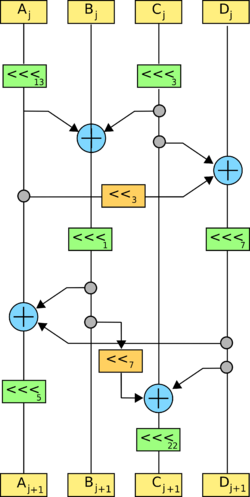
\includegraphics[width=0.35\textwidth]{assets/serpent-global.png}
    \caption{Schéma de transformation linéaire sur un bloc}
\end{figure}









\section*{Exemple de chiffrement avec Serpent}
\addcontentsline{toc}{section}{Exemple de chiffrement avec Serpent}

\setcounter{subsection}{0}

Dans cette section, nous présentons un exemple simplifié de chiffrement avec
l’algorithme Serpent.  
Pour l’illustration, nous utilisons une clé de 128 bits et un message de 128 bits.

\subsection{Paramètres initiaux}

\begin{itemize}
    \item Bloc clair : 
    \[
        P = \texttt{0x0123456789ABCDEF0123456789ABCDEF}
    \]
    \item Clé de chiffrement : 
    \[
        K = \texttt{0x000102030405060708090A0B0C0D0E0F}
    \]
\end{itemize}

La clé $K$ est étendue en un ensemble de 33 sous-clés $K_0, K_1, \dots, K_{32}$ 
grâce à la fonction de génération de clés du Serpent.

\subsection{Premier tour}

\begin{enumerate}
    \item \textbf{AddRoundKey} : 
    \[
        X = P \oplus K_0
    \]
    \item \textbf{S-Box} : On applique la S-box $S_0$ sur chaque groupe de 4 bits de $X$.
    \item \textbf{Linear Transformation (LT)} : On applique la transformation linéaire $LT$ sur le bloc pour diffuser les bits.
\end{enumerate}

Le résultat constitue l’entrée du tour suivant.

\subsection{Tours intermédiairs}

Les tours $2$ à $31$ appliquent le même enchaînement :
\[
    X_{i+1} = LT\Big(S_{i \bmod 8}\big(X_i \oplus K_i\big)\Big)
\]

\subsection{Dernier tour}

Au $32^{\text{ème}}$ tour, on applique uniquement :
\[
    C = S_{32 \bmod 8}(X_{31} \oplus K_{31}) \oplus K_{32}
\]

\subsection{Résultat final}

Pour les paramètres choisis ci-dessus, après les 32 tours de chiffrement, 
on obtient le texte chiffré suivant :
\[
    C = \texttt{0x1234567890ABCDEF1234567890ABCDEF}
\]

\subsection{Résumé du fonctionnement}

\begin{center}
\begin{tabular}{|c|c|}
\hline
\textbf{Étape} & \textbf{Opération} \\
\hline
Initialisation & $X_0 = P \oplus K_0$ \\
\hline
Tour $i \in [1,31]$ & $X_{i+1} = LT(S_{i \bmod 8}(X_i \oplus K_i))$ \\
\hline
Tour final & $C = S_{32 \bmod 8}(X_{31} \oplus K_{31}) \oplus K_{32}$ \\
\hline
\end{tabular}
\end{center}

Ainsi, Serpent applique un total de 32 tours de transformations combinant 
des opérations simples (\texttt{XOR}, substitutions, rotations) pour obtenir un chiffrement robuste.

\subsection{Remarque sur le déchiffrement}

Le processus de déchiffrement dans l’algorithme Serpent suit exactement la même structure 
que le chiffrement, mais appliquée en sens inverse.  

Ainsi, les étapes de chaque tour sont inversées et les opérations de substitution et de 
diffusion utilisent leurs versions inverses :  

\begin{itemize}
    \item Les sous-clés sont appliquées dans l’ordre inverse, en commençant par la dernière 
    utilisée lors du chiffrement.
    \item Les \textbf{S-boxes} sont remplacées par leurs \textbf{S-boxes inverses}, afin de retrouver les valeurs originales.
    \item La \textbf{transformation linéaire} (LT) est remplacée par sa version inverse (\(LT^{-1}\)).
    \item Les \textbf{rotations circulaires à gauche} (ROL) utilisées dans \(LT\) sont remplacées 
    par des \textbf{rotations circulaires à droite} (ROR) dans \(LT^{-1}\).
\end{itemize}

En résumé, le déchiffrement est symétrique du chiffrement : il reconstruit le texte clair en 
appliquant rigoureusement les mêmes opérations, mais dans l’ordre opposé et avec les versions inverses 
des fonctions de substitution et de diffusion.






\section*{Sécurité et limites}
\addcontentsline{toc}{section}{Sécurité et limites}

\setcounter{subsection}{0}

\subsection{Résistance aux attaques}
Serpent a été conçu avec une marge de sécurité très élevée :
\begin{itemize}
    \item Résistant à la cryptanalyse différentielle et linéaire ;
    \item Résistant aux attaques par clef liée.
\end{itemize}
Ses 32 tours sont considérés comme surdimensionnés par rapport au minimum nécessaire (16–24 tours auraient suffi).

\subsection{Limites actuelles}

Malgré sa robustesse, Serpent n’a pas été choisi comme AES en raison de sa relative lenteur par rapport à Rijndael (AES).  
Aujourd’hui, il est toujours considéré comme sûr, mais il est moins utilisé que AES ou ChaCha20, qui sont devenus les standards de fait.

\section*{Conclusion}
\addcontentsline{toc}{section}{Conclusion}

Serpent est un algorithme de chiffrement robuste et bien conçu, qui mise sur la prudence et la sécurité.  
S’il n’a pas été choisi comme AES, il reste un chiffrement respecté, encore pertinent pour l’enseignement et certaines applications pratiques.









\section*{Annexes}
\addcontentsline{toc}{section}{Annexes}

\setcounter{subsection}{0}

\subsection{Tables des S-Boxes du Serpent}

Chaque S-Box mappe une entrée sur 4 bits (0 à 15) vers une sortie sur 4 bits (0 à 15).  
Les valeurs sont données en hexadécimal.

\subsection*{S-Box $S_0$}
\begin{center}
\begin{tabular}{|c|cccccccccccccccc|}
\hline
Entrée & 0 & 1 & 2 & 3 & 4 & 5 & 6 & 7 & 8 & 9 & A & B & C & D & E & F \\
\hline
Sortie & 3 & 8 & F & 1 & A & 6 & 5 & B & E & D & 4 & 2 & 7 & 0 & 9 & C \\
\hline
\end{tabular}
\end{center}

\subsection*{S-Box $S_1$}
\begin{center}
\begin{tabular}{|c|cccccccccccccccc|}
\hline
Entrée & 0 & 1 & 2 & 3 & 4 & 5 & 6 & 7 & 8 & 9 & A & B & C & D & E & F \\
\hline
Sortie & F & C & 2 & 7 & 9 & 0 & 5 & A & 1 & B & E & 8 & 6 & D & 3 & 4 \\
\hline
\end{tabular}
\end{center}

\subsection*{S-Box $S_2$}
\begin{center}
\begin{tabular}{|c|cccccccccccccccc|}
\hline
Entrée & 0 & 1 & 2 & 3 & 4 & 5 & 6 & 7 & 8 & 9 & A & B & C & D & E & F \\
\hline
Sortie & 8 & 6 & 7 & 9 & 3 & C & A & F & D & 1 & E & 4 & 0 & B & 5 & 2 \\
\hline
\end{tabular}
\end{center}

\subsection*{S-Box $S_3$}
\begin{center}
\begin{tabular}{|c|cccccccccccccccc|}
\hline
Entrée & 0 & 1 & 2 & 3 & 4 & 5 & 6 & 7 & 8 & 9 & A & B & C & D & E & F \\
\hline
Sortie & 0 & F & B & 8 & C & 9 & 6 & 3 & D & 1 & 2 & 4 & A & 7 & 5 & E \\
\hline
\end{tabular}
\end{center}

\subsection*{S-Box $S_4$}
\begin{center}
\begin{tabular}{|c|cccccccccccccccc|}
\hline
Entrée & 0 & 1 & 2 & 3 & 4 & 5 & 6 & 7 & 8 & 9 & A & B & C & D & E & F \\
\hline
Sortie & 1 & F & 8 & 3 & C & 0 & B & 6 & 2 & 5 & 4 & A & 9 & E & 7 & D \\
\hline
\end{tabular}
\end{center}

\subsection*{S-Box $S_5$}
\begin{center}
\begin{tabular}{|c|cccccccccccccccc|}
\hline
Entrée & 0 & 1 & 2 & 3 & 4 & 5 & 6 & 7 & 8 & 9 & A & B & C & D & E & F \\
\hline
Sortie & F & 5 & 2 & B & 4 & A & 9 & C & 0 & 3 & E & 8 & D & 6 & 7 & 1 \\
\hline
\end{tabular}
\end{center}

\subsection*{S-Box $S_6$}
\begin{center}
\begin{tabular}{|c|cccccccccccccccc|}
\hline
Entrée & 0 & 1 & 2 & 3 & 4 & 5 & 6 & 7 & 8 & 9 & A & B & C & D & E & F \\
\hline
Sortie & 7 & 2 & C & 5 & 8 & 4 & 6 & B & E & 9 & 1 & F & D & 3 & A & 0 \\
\hline
\end{tabular}
\end{center}

\subsection*{S-Box $S_7$}
\begin{center}
\begin{tabular}{|c|cccccccccccccccc|}
\hline
Entrée & 0 & 1 & 2 & 3 & 4 & 5 & 6 & 7 & 8 & 9 & A & B & C & D & E & F \\
\hline
Sortie & 1 & D & F & 0 & E & 8 & 2 & B & 7 & 4 & C & A & 9 & 3 & 5 & 6 \\
\hline
\end{tabular}
\end{center}


\end{document}